% This file is the Latex source of the Big Data course project
% report. The project contributors are Ali Alavi, Rolf jagerman
% and Ken Tsay.
% The report is written by Ali Alavi, Rolf Jagerman.

%
\documentclass{llncs}
%

\usepackage{graphicx} % for importing images
\usepackage{caption}
\usepackage{subcaption} % for subfigures
\captionsetup{compatibility=false} % to make subfigures compatible with template

\usepackage{url} % for URL references
\urlstyle{same}
\usepackage{float} % helps with locating the 
\usepackage[T1]{fontenc}  % providing font encoding
% used for drawing the diagrams
%
\begin{document}
%
\mainmatter              % start of the contributions
\pretolerance=10000  % This avoids long lines
\pagestyle{headings}
%\hyphenation{}

%
\title{Automatic News Generation Based on Twitter}
%
\titlerunning{Automatic News Generation Based on Twitter}  % abbreviated title (for running head)
%                                     also used for the TOC unless
%                                     \toctitle is used
%
\author{Ali Alavi\inst{1} \and Rolf Jagerman\inst{1} \and
Tsay Kai-En\inst{1}}
%
\authorrunning{Ali Alavi, Rolf Jagerman and Tsay Kai-En} % abbreviated author list (for running head)
%
%
\institute{ETH Z\"urich, Z\"urich, Switzerland\\
\email{alavis@ethz.ch, \{rolfj, tsayk\}@student.ethz.ch}
}

\maketitle              % typeset the title of the contribution
%

\section{Introduction}
% todo
This report presents the current status of the project \textbf{Automatic News Generation Based on Twitter}, for the \textbf{Big Data} course (code \textit{263-3010-00L}). This project tries to answer the following questions: 
\textit{Can we automatically generate news headlines based on public twitter posts? Can this method of news generation perform better than the available news agencies, in terms of speed, reliability and so on?}

We tackle this problem by taking the following steps:

\begin{enumerate}
	\item \textit{Data collection: }Gathering a large set of twitter posts and news headlines 
	\item \textit{Building a classifier: }Use the news headlines to train a classifier
	\item \textit{Labeling the tweets: }Label each tweet using the classifier
	\item \textit{Post-processing tweets: }Find term-frequencies over time to detect news trends
\end{enumerate}

A big picture of the system is depicted in Figure \ref{fig:A big picture of the system}. In the rest of this report we will elaborate on how we implemented the solution in a scalable way using Apache Spark.

\begin{figure}[H]
	\centering
	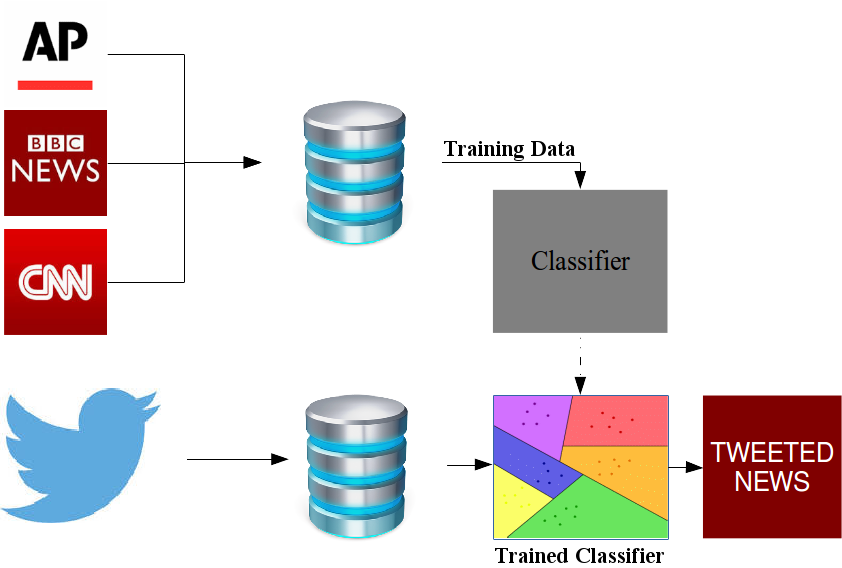
\includegraphics[width=0.8\textwidth]{images/bigpicture.png} 
	\caption{A big picture of the system}
	\label{fig:A big picture of the system}
\end{figure}



\section{Data model}
The twitter streaming API provides data in JSON format. It outputs a tweet as a JSON object on a single line. We copied this data storage format to our permanent data storage. That is: we have a JSON object representing a tweet on each separate line in our data files.

The Spark Map-Reduce framework naturally works with text data where each line represents a new element. By using functionality such as Spark's \texttt{textFile}, we can map each line of text, which represents a tweet, to a specific function. This makes using the data in a Map-Reduce context extremely easy.

\section{Design of the system}
The system architecture is depicted in Figure \ref{fig:architecture}. The main idea here is to train a classifier for several news topics using the news twitter accounts as training data. Then we use this classifier to predict the massive stream of public tweets into these news topics. Any tweets that are not classified as 'sports', 'politics' or 'technology' are discarded. This filters out most of the non-relevant tweets. Finally the predicted tweets are used to compute term frequencies over time and detect interesting news trends.

\begin{figure}[H]
	\centering
	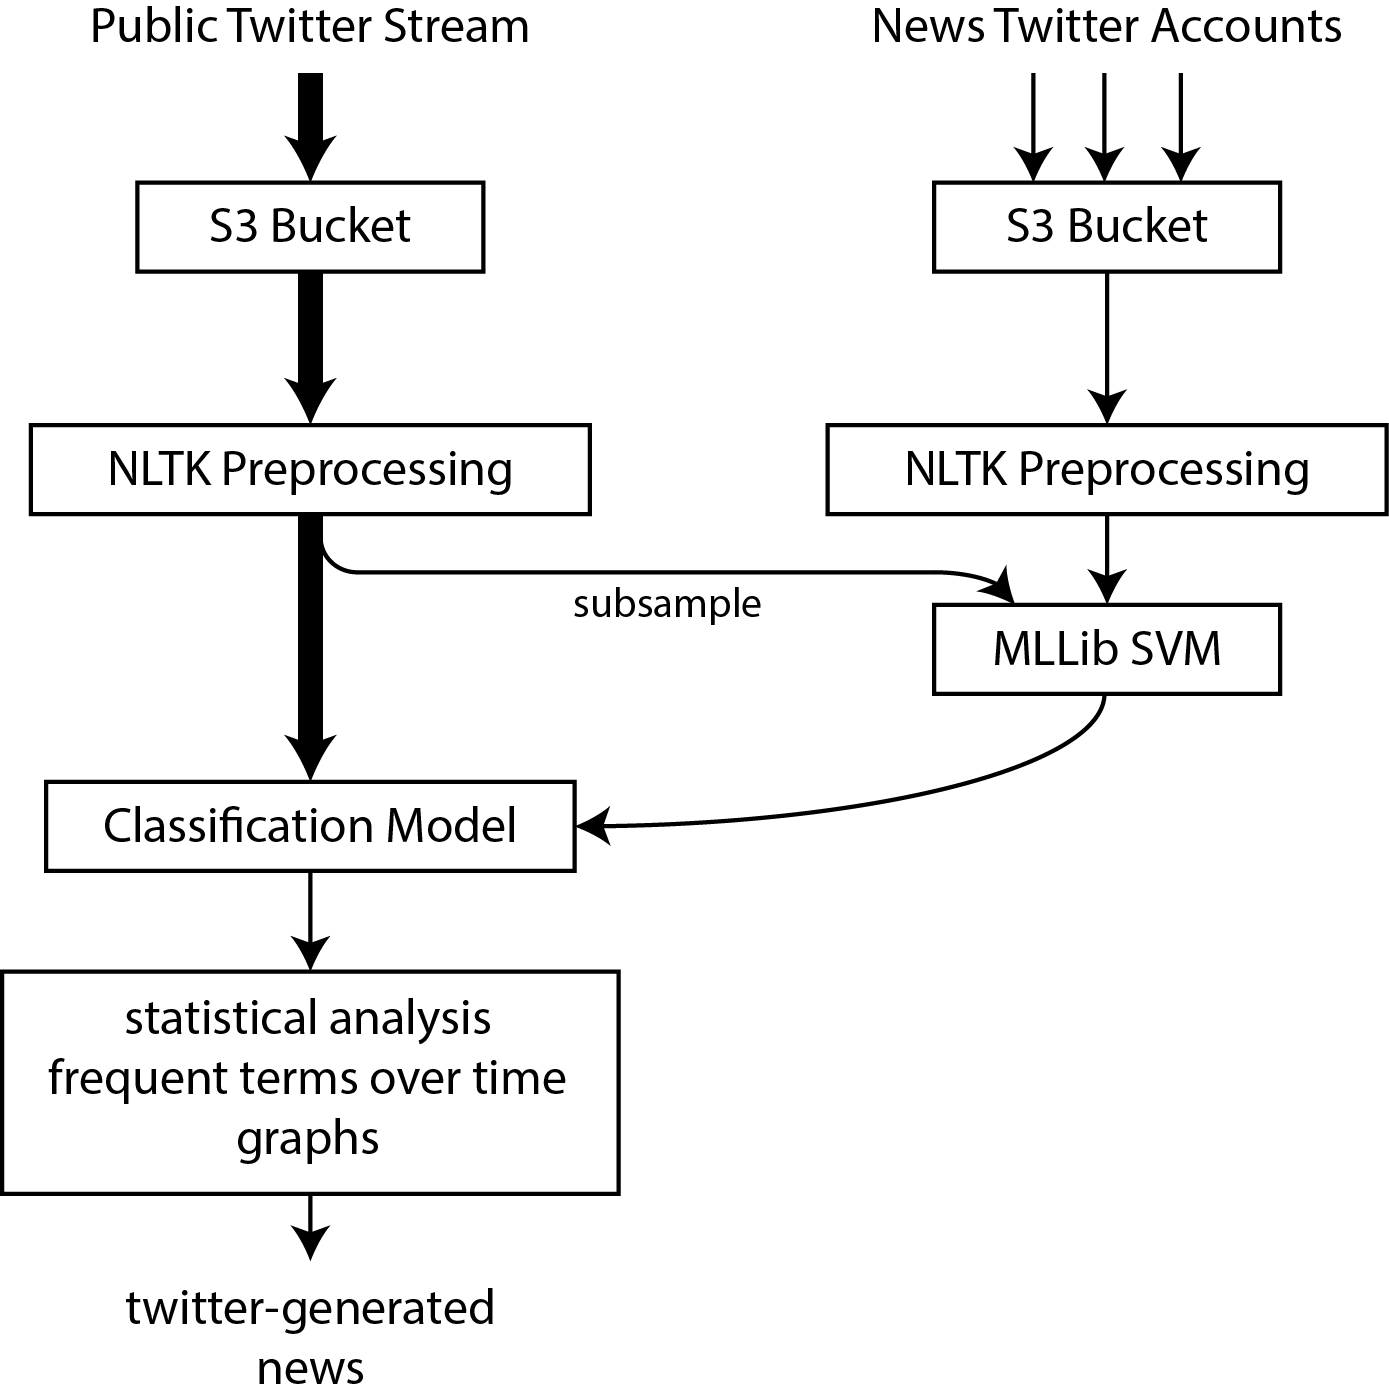
\includegraphics[width=0.72\textwidth]{images/system_arch.png} 
	\caption{The architecture of the system}
	\label{fig:architecture}
\end{figure}

\subsection{Data storage}
We stored around 600GB of the twitter stream data on Amazon S3. We used the s3cmd tool, which is a command line tool and client for uploading, retrieving and managing data in Amazon S3 \cite{s3cmd}. By integrating our data collection script with this tool, we can directly upload the twitter streaming data into the S3 bucket. This benefits the whole system because we can load the large data set using the S3 protocol into our Spark instances.

\subsection{Data processing platform}
The data processing platform we use is Apache Spark running on top of Amazon Elastic MapReduce (EMR). Initially we ran Spark on Amazon EC2 directly without using EMR. It turned out that the default configuration did not work well, and the executed tasks had a failure rate of 25\% - 50\%. For this reason, we decided to try the EMR platform. This platform has Spark pre-configured, which resulted in a 0\% failure rate for our tasks.

\subsection{Classification}
We want to classify the tweets into the three possible news-topics 'sports', 'technology' and 'politics'. The data preprocessing is done using NLTK \cite{nltk} and Scikit-Learn \cite{scikit-learn}. We use the default NLTK word tokenizer and stem each token using the Lancaster stemmer. Additionally we generate bigrams and trigrams of the text data. We use Scikit-Learn to generate sparse feature vectors by hashing each token to a feature. The final classification model is an SVM with $L_1$ regularization, trained using Spark's MLLib library\cite{mllib}.

\subsection{Post-processing predicted tweets}
\label{sec:postprocess}
Although the classifier manages to classify the tweets in the mentioned categories, these classified outputs are not essentially news headlines. This is due to the fact that the classifier classifies the tweets individually, while an important property of news-related tweets is their frequency of appearance in a given timeframe. Hence, we need to perform some temporal analysis of the classified tweets.

We perform analysis by sampling the predicted tweets, with a rate of \textit{R}, then tokenizing the classified tweets and filtering out the less frequent nouns. In this way, we manage to filter out lots of noisy outputs of the classifier. Afterwards, we look into different slope of the time series, and identify top surging topics as news-worthy topics, which can be presented to the users.


\section{Results}

\subsection{Classification performance}

In our previous report, we measured our news classifier's performance by using precision, recall and f1-score. These scores are shown in table \ref{tbl:oldclassifier}.

\begin{table}
	\begin{center}
		\begin{tabular}{|r|r|r|r|r|} \hline
			class  & precision   & recall & f1-score  & support \\ \hline
			technology    &   1.00 &     0.08  &    0.14   &   6195 \\
			sports   &    1.00   &   0.03   &   0.07   &   6365 \\
			politics   &    1.00  &    0.10   &   0.18   &   6376 \\
			avg / total  &     1.00   &   0.07  &    0.13   &  18936 \\ \hline
		\end{tabular}
	\end{center}
	\caption{Old classification performance over the three trained categories}
	\label{tbl:oldclassifier}
\end{table}

It was evident that the classifier was not performing optimally. The high precision measures were offset by the extremely low recall measures. This meant that the classifier was only predicting the relevant labels for a few tweets and discarding most of them. This was likely the result of training on an imbalanced data set.

The new classifier was trained on roughly two to three times as much data. Additionally, we ensured that each classifier in the one-vs-all approach was trained on roughly equally many positive and negative data samples. The scores for this new balanced classifier is shown in table \ref{tbl:newclassifier}

\begin{table}
	\begin{center}
		\begin{tabular}{|r|r|r|r|r|} \hline
			class  & precision   & recall & f1-score  & support \\ \hline
			technology    &   0.78 &     0.92  &    0.84   &  25343 \\
			sports   &    0.75   &   0.73   &   0.74   &   25343 \\
			politics   &    0.83  &    0.75   &   0.79   &   25343 \\
			avg / total  &     0.79   &   0.80  &    0.79   &  76029 \\ \hline
		\end{tabular}
	\end{center}
	\caption{New classification performance over the three trained categories}
	\label{tbl:newclassifier}
\end{table}

Although the precision of the classifier has gone down, our recall has increased significantly. This means that, although some predictions are wrong, we have a lot more predictions to work with. This benefits the post-processing step where we use term frequencies over time to determine news trends.

Despite scaling up the entire system, the amount of available training data did not increase significantly. The changes in performance are not due to an increase of data, but are more likely attributed to training on a more balanced data set.

\subsection {Post-processing the classified results}
Selecting the sampling rate $R$ (as mentioned in section \ref{sec:postprocess}) is non-trivial, as it depends on the life time of each news item, which varies based on the news topic, scale (global or regional), and so on. Despite that, we managed to obtain reasonable results with sampling frequencies of 1 hour. For example, in Figure \ref{fig:Political news topic prediction using time series analysis, with a sampling frequency of 1 hour} we see that the two most common topics are Obama and immigration. This corresponds to the recent announcement by Obama on the change of immigration laws.

\begin{figure}
	\centering
	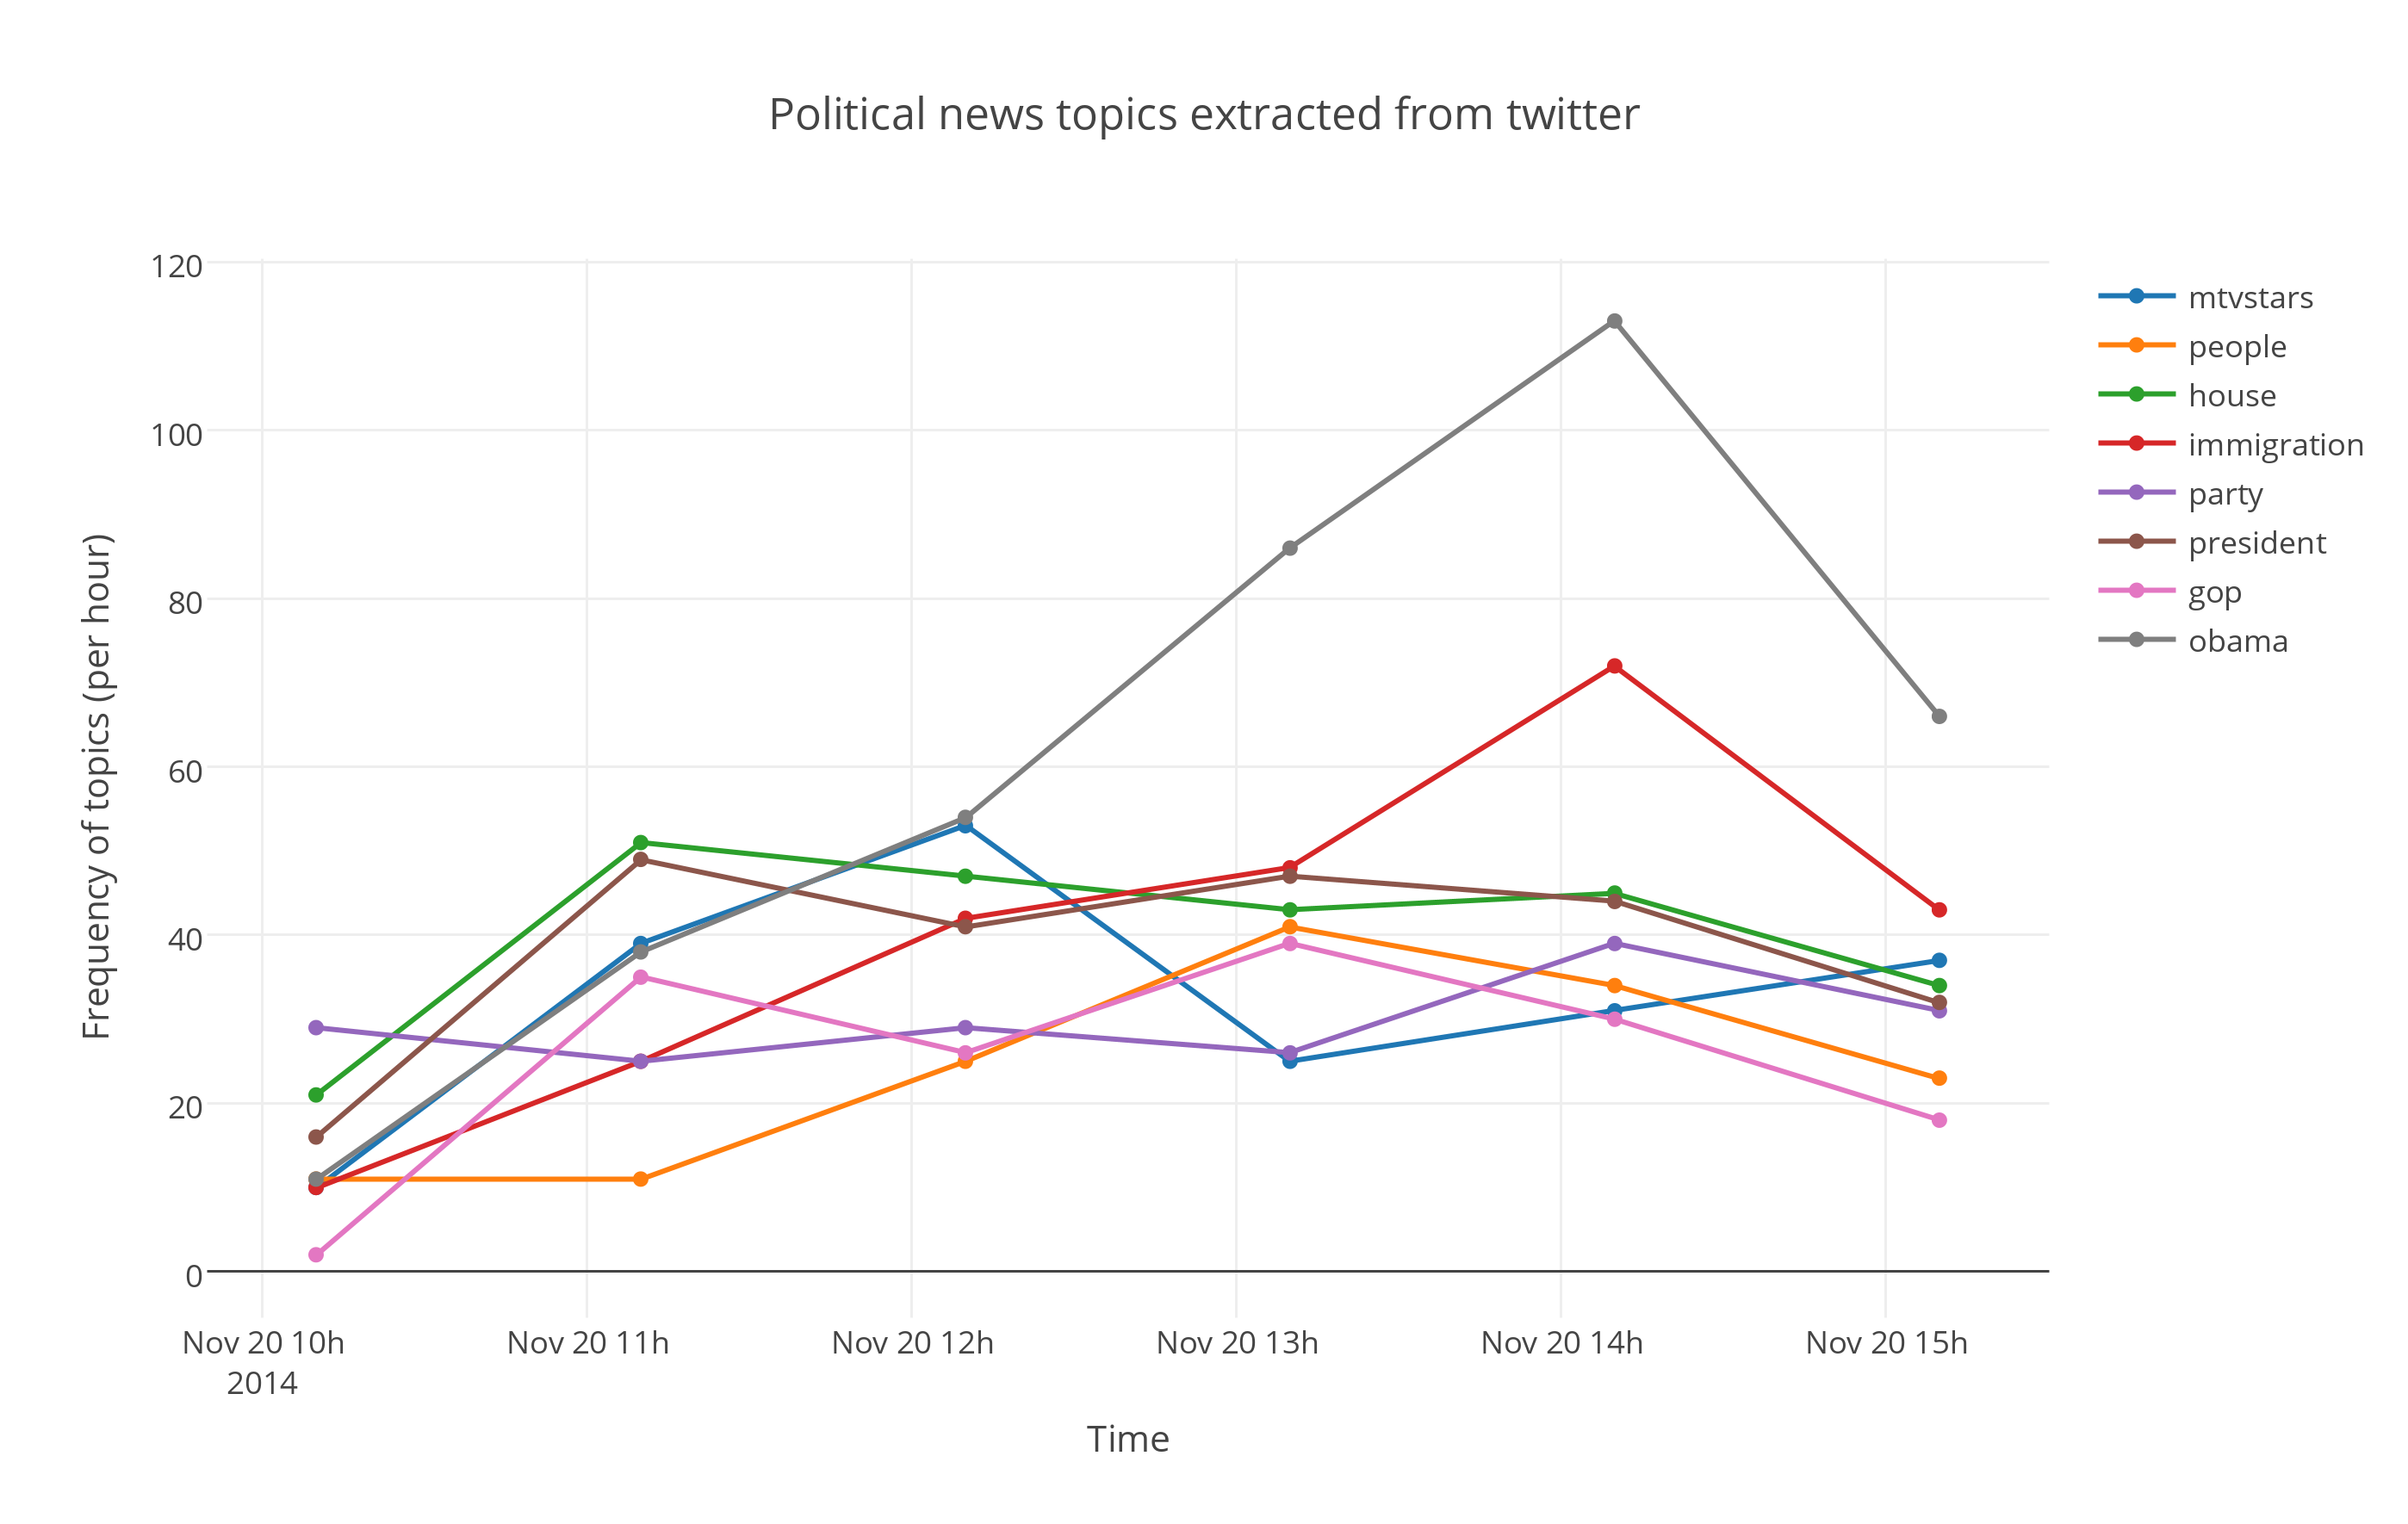
\includegraphics[width=0.8\textwidth]{images/political_news_topics_extracted_from_twitter.png} 
	\caption{Political news topic prediction using time series analysis, with a sampling frequency of 1 hour}
	\label{fig:Political news topic prediction using time series analysis, with a sampling frequency of 1 hour}
\end{figure}

\subsection{Prediction scalability}

We were able to classify 600GB of tweets in roughly 10 hours using 20 Amazon EC2 m1.medium instances. The Spark Map-Reduce framework created 10,702 tasks. Each of these tasks independently computes the predictions on a part of the dataset and write the results to a file on S3. A single task takes on average $65.4 (\pm 20.6)$ seconds to complete. Since we were restricted to a maximum of 20 EC2 instances, this takes about 10 hours in total.

\section{Conclusion}
Our main goal in this part of the project was to scale up our prediction capability. We want to use our trained classifier to quickly classify all of the collected tweets. We have succeeded in doing so and the final performance of the system is satisfactory. Our Amazon account was limited to a maximum of 20 EC2 instances. Without this limitation and with a sufficient number of instances, the computations on our big data set could have finished in minutes rather than hours.

\bibliographystyle{plain}
\bibliography{report.bib}

\end{document}